\section{Rejection as a negative margin}
\label{sec:theory}

Throughout, $g = \max_{j \ne y} p_j - p_y \in (-1, 1)$ is the \emph{label gap}: $g < 0$ when
the training label is the model's top class, and $g > 0$ when some other class beats it. All
statistics below are computed under stop-gradient, as the mask is. Proofs are in
\cref{app:proofs}. Every closed-form number quoted in this section is checked against the code in
\texttt{tests/test\_mechanism.py}.

\subsection{The zero-loss region}

\begin{proposition}[Zero loss $\Leftrightarrow g \le -\delta$]
\label{prop:zero}
For any $\delta \in [-1, 1]$, the masked loss \eqref{eq:masked} satisfies
$\ell_\delta(o, y) = 0 \iff \nabla_o \ell_\delta(o, y) = 0 \iff g \le -\delta$.
If $g > -\delta$, the leading competitor $j^\star = \arg\max_{j\ne y} p_j$ is in $K_\delta$ and
$\ell_\delta > 0$.
\end{proposition}

For $\delta > 0$ this is AS-Softmax's sparsity: a sample stops contributing once its label wins by
at least $\delta$ (\emph{fitted}). For $\delta < 0$ the zero-loss region extends past $g = 0$: a
sample whose label is beaten by up to $|\delta|$ also contributes nothing (\emph{rejected}).
Nothing in the loss distinguishes the two cases. The same exact zero that makes AS-Softmax sparse
is the zero of a discarded sample.

\begin{corollary}[Selection rules are margins]
\label{cor:selection}
Any per-sample keep/reject decision $a_i \in \{0, 1\}$ is realized by $\delta_i = 1$ if $a_i = 1$
and $\delta_i = -1$ otherwise: kept samples train with cross-entropy and rejected ones contribute
nothing. In particular, small-loss selection with forget rate $r$ is the binary margin
$\delta_i = 1 - 2\,\mathbb{1}[\text{sample $i$ is among the $\lceil rB \rceil$ highest-loss samples of
its batch}]$, up to the normalization of the batch mean.
\end{corollary}

\subsection{A family of suspicion margins}

Small-loss uses two margin values. A smooth family interpolates between AS-Softmax and rejection.

\begin{definition}[Suspicion margin]
\label{def:family}
Given a per-sample suspicion statistic $s_i \in (0, 1)$ ($s_i > 1/2$: suspicious), a base margin
$\dbase$, a ceiling $\dceil \ge \dbase$ and a strength $\beta(t) \ge 0$,
\[
  \delta_i = \clip\!\big(\dbase - \beta(t)\,(2 s_i - 1),\; -1,\; \dceil\big).
\]
\end{definition}

We use $\dbase = \dceil = 0.15$, the AS-Softmax value. The ceiling makes the family one-sided: a
confident sample never trains under a tighter margin than AS-Softmax would give it. $\beta(t)$
ramps linearly from 0 to $\beta$ over the first 30\% of training and then holds, the shape of
Co-teaching's forget-rate schedule. $\beta = 0$ is AS-Softmax. We study three statistics:
\begin{itemize}
  \item \textbf{batch-relative} (``M4''): $s_i = \sigma(z_i / T)$ with
  $z_i = (\bar p_y - p_{y,i}) / \mathrm{sd}_B(p_y)$, the z-score of the label probability within
  the mini-batch;
  \item \textbf{absolute gap}: $s_i = \sigma(g_i / \tau)$, suspicious iff another class currently
  beats the label;
  \item \textbf{loss mixture}: the posterior of the high-loss component of a two-component Gaussian
  mixture fitted to per-sample running log-losses, as in DivideMix (\cref{app:mixture}).
\end{itemize}

\begin{proposition}[Rejection condition and the escape region]
\label{prop:reject}
Under \cref{def:family}, sample $i$ has zero loss iff
\[
  g_i \le -\dceil \quad\text{(fitted)} \qquad\text{or}\qquad
  \beta\,(2 s_i - 1) \ \ge\ \dbase + g_i \quad\text{(rejected)}.
\]
Consequently, a sample with $g_i \ge \beta - \dbase$ is never rejected, whatever its statistic,
and trains against at least its leading competitor $j^\star$.
\end{proposition}

The cap $\beta - \dbase$ explains why memorization responds to $\beta$ as a threshold
(\cref{fig:geometry}b). With $\dbase = 0.15$, strengths $\beta = 0.25, 0.5, 1$ can reject only
samples whose label trails by less than $0.10, 0.35, 0.85$. Once early learning has made the model
confident in the true class of a mislabeled sample, its gap is large. A small $\beta$ then rejects
almost none of the noise. At 40\% symmetric noise the three strengths end training with 96\%,
54\% and 16\% of corrupted labels memorized; AS-Softmax ($\beta = 0$) reaches 96\%
(\cref{tab:main}). The escape region also has a cost of its own. A confidently contradicted
label, the clearest case of label noise, then receives a near-maximal per-sample gradient toward
the wrong label. Under the absolute statistic below it is binary cross-entropy against $j^\star$
alone, with $\ell_1$-norm $2(1 - p_y/(p_y + p_{j^\star})) \approx 2$.

\begin{figure}[t]
  \centering
  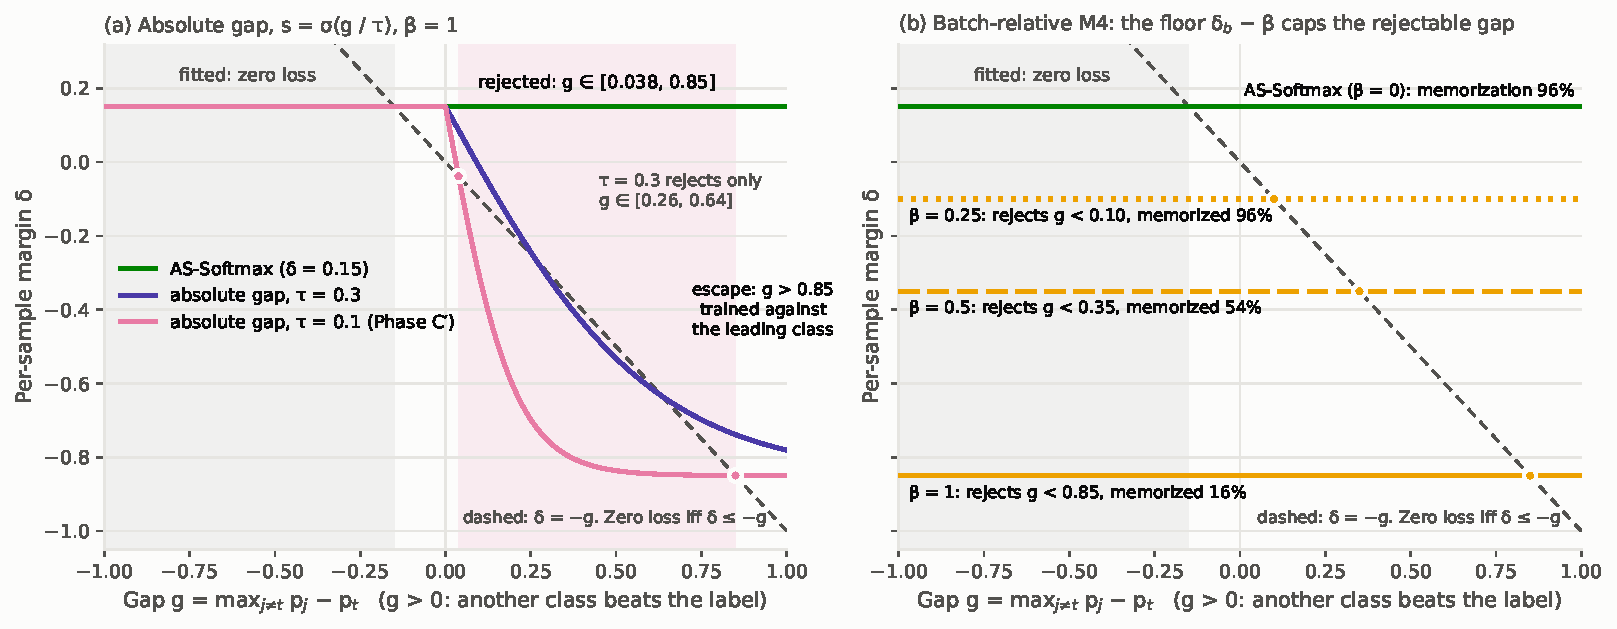
\includegraphics[width=\linewidth]{figures/fig1_geometry.pdf}
  \caption{Margin geometry. A sample has zero loss iff its margin lies on or below the dashed
  line $\delta = -g$ (\cref{prop:zero}). (a)~The absolute-gap margin rejects a fixed band of gaps,
  $[0.038, 0.85]$ at $\tau = 0.1$ and only $[0.26, 0.64]$ at $\tau = 0.3$, independent of the noise
  rate (\cref{cor:band}). Above $g_{\mathrm{hi}}$ the sample escapes rejection. (b)~The batch-relative
  margin can reach no lower than $\dbase - \beta$, so it can only reject gaps below $\beta - \dbase$
  (\cref{prop:reject}). The memorization figures are from \cref{tab:main} (40\% symmetric noise,
  last epoch).}
  \label{fig:geometry}
\end{figure}

\subsection{Batch-relative statistics are blind to the noise rate}

\begin{proposition}[Affine invariance]
\label{prop:blind}
Let $s_i = h(z_i)$ for an increasing function $h$ of the batch z-score $z_i$ of $p_{y,i}$. Replacing every
$p_{y,i}$ in the batch by $a\,p_{y,i} + b$ with $a > 0$ leaves every $s_i$ unchanged. The fraction
of the batch with $s_i \ge h(k)$, $k > 0$, is at most $1/(1+k^2)$, and the fraction with
$z_i > 0$ is the fraction below the batch mean, whatever the share of wrong labels in the batch.
\end{proposition}

A batch with 40\% wrong labels and a clean batch at an earlier stage of training can have the same
standardized distribution of $p_y$, and then receive the same suspicion scores. The statistic
measures \emph{relative} fit only. It flags roughly the lower half of every batch, and how much of
that half is rejected is set by $\beta$ through \cref{prop:reject}, not by the data. The method
therefore carries a fixed rejection rate that nobody chose explicitly. It suits one noise level
and over- or under-rejects everywhere else. On clean data it discards correctly labeled samples
that are merely below average (\cref{sec:results}). Small-loss selection has the same
blindness by construction. There the rate is an explicit input $r$, typically set to the true
noise rate, which is information the method should not need.

\subsection{An absolute statistic gives a rate-free rejection band}

\begin{corollary}[Rejection band]
\label{cor:band}
With $s_i = \sigma(g_i / \tau)$ and full strength $\beta$, the rejected gaps are
\[
  R = \{\, g > 0 : \beta \tanh\!\big(g / 2\tau\big) \ge \dbase + g \,\},
\]
an interval $[g_{\mathrm{lo}}, g_{\mathrm{hi}}]$ (possibly empty) that depends on
$(\beta, \tau, \dbase)$ alone. For $\beta = 1$, $\dbase = 0.15$:
$R = [0.038, 0.850]$ at $\tau = 0.1$ and $R = [0.265, 0.635]$ at $\tau = 0.3$.
\end{corollary}

The band involves neither the batch, nor the noise rate, nor an estimate of either. What the rule
rejects follows the data: on clean data, once the model fits, few samples have $g > 0$ and few are
rejected; under heavy noise, many are. The rule is rate-free, not parameter-free. Its three
constants fix the band in advance, and \cref{fig:geometry}a shows that the scale matters: at
$\tau = 0.3$ the band shrinks to $[0.26, 0.64]$, the most contradicted labels escape, and
memorization stays at the level of plain AS-Softmax (96\%, \cref{tab:main}). The absolute rule
trains on two regions: near-ties, $g \in (-\dceil, g_{\mathrm{lo}})$, and the escape region
$g > g_{\mathrm{hi}}$.

\subsection{AS-Softmax and memorization}

\begin{observation}
\label{obs:as}
Cross-entropy gives every sample a logit gradient of $\ell_1$-norm $2(1 - p_y) > 0$. AS-Softmax
gives exactly zero to every fitted sample, $g \le -\dbase$. As clean samples become fitted, a larger
share of each update comes from the samples that are not, and once early learning is over most of
those carry wrong labels. Adam's per-coordinate normalization \citep{kingma2015adam,loshchilov2019adamw} makes
the step size largely insensitive to the overall gradient scale. We therefore expect AS-Softmax to
memorize corrupted labels faster than cross-entropy in mid-training, with both saturating
eventually.
\end{observation}

The observation is a prediction, not a theorem. \Cref{sec:mechanism} measures both the
memorization curves and the share of gradient carried by mislabeled samples.
